\chapter{Organization Overview} % Background \& Literature Overview
\label{chap:org}
\textbf{In this section we'll review Tunisie Telecom's History, Notable Leaders, Its' business sector and the wide range of clients it offers its services to, as well as its' organizational hierarchy and it's work environment.}
\section{Introduction to Tunisie Telecom \& History} % Some Technique One
\index{Introduction to Tunisie Telecom \& History|(}%%Some Technique One

%\blindtext
\index{Introduction to Tunisie Telecom \& History!Introduction to TT}%%Some Sub-technique One%make it the subsection name
%\blindtext
\subsection{Introduction to TT}%Some Sub-sub-technique One
Tunisie Telecom is the brand name of the historical provider of telecommunication services in Tunisia. Its capital is 875 million euros and its transaction number, in 2004, amounted to 750 million euros.

Tunisie Telecom is the fully integrated telecom services operator in Tunisia, with leading market positions across all segments with over 7 million customers and an employee base of c.7,500. Tunisie Telecom offers the largest mobile coverage in the country, owns and operates a nationwide fixed and fiber network infrastructure. This is complemented by an extensive submarine cable network allowing for direct and fully redundant connectivity with Europe, Africa and Asia. Tunisie Telecom’s service offering ranges from 4G mobile broadband to Fiber-To-The-Home and Fiber-To-The-Building as well as cloud and IP-MPLS solutions for entreprises.
%\textbf{Comment: Find more recent data}

\index{Introduction to Tunisie Telecom \& History!History}%%Some Sub-sub-technique One%make it the subsection name to which you want to jump
%\blindtext
\subsection{History} %% %% %% PAST TENSE ???
The law establishing the National Telecommunications Office, whose commercial name is Tunisie Télécom, was promulgated on 17 April 1995 and came into force on 1 January 1996.

Tunisie Télécom sets up, operates and markets the first GSM network in Mauritania (Mattel) from May 2000. It also enters into a technical cooperation agreement with Djibouti Telecom for the development of its telecommunications networks.

It became a public limited company at the end of 2002, it changes its legal status, by a decree of April 5, 2004, to become a limited company called "Tunisie Telecom". It is experiencing partial privatization in July 2006 with the entry into its capital, up to 35\%, of the Emirati consortium EIT (Emirates International Telecommunications).

From 2008, Tunisie Telecom offers the possibility to national bank card holders to feed the balance of their prepaid lines via ATMs of the Arab Tunisian Bank (Mobilink service).

On March 21, 2009, Tunisie Telecom launched a new brand, Elissa, with offers specifically designed for young people under 25; it becomes accessible to all without age limit as of March 10, 2012.

In the spring of 2011, following the Tunisian revolution, the company is shaken by a major social conflict between the representatives of the Tunisian General Labor Union (UGTT) and those of its UAE shareholder over the fate of some 60 contracts representing 3.5\% of the payroll; it is marked by strikes and sit-ins affecting the proper functioning of the operator. It ends with the end of these employment contracts, with the exception of ten contract holders retaining their positions.

In September 2012, Chief Executive Officer (CEO) Ali Ghodhbani retires and is replaced by Mokhtar Mnakri, former CEO of Alcatel's subsidiary.

In 2014, Salah Jarraya was appointed CEO to replace Mnakri, whose term was coming to an end.

In June of the same year, the employees started a social movement to obtain a salary increase and to claim the application of the agreements signed in February 2011. They gather around the UGTT and carry out many work stoppages until May they succeed in May 2015. Following these social movements and strikes, Jarraya resigns on July 2nd.

On August 12, Nizar Bouguila is appointed CEO.

On March 15, 2016, Tunisie Telecom launched its new visual identity called "Life is Emotions", with a new logo. In August, Tunisie Telecom finalizes the purchase of 65.4\% of the entire capital of GO.

Bouguila is replaced on September 19, 2017 by Mohamed Fadhel Kraiem. On November 7, Tunisie Telecom signed a five-year contract with the Ministry of Information Technologies and the Digital Economy to cover white areas with broadband telecommunications services.

On December 13, 2017, UAE investment fund Abraaj announced that it had signed an agreement the day before for the definitive purchase of EIT's 35\% stake. However, the bankruptcy of the fund cancels the operation.




%\blindtext

%\blindtext
\index{Introduction to Tunisie Telecom \& History|)}

% \section{Global Leaders of Tunisie Telecom}%[Some Technique Two]{Some Technique Two with Super Long Title Which Will Overrun In Header}
% \index{Global Leaders of Tunisie Telecom|(}%%Some Technique Two
% %\blindtext[5]
% Ali Ghodhbani - Mokhtar Mnakri - Salah Jarraya - Nizar Bouguila - Mohamed Fadhel Kraiem %% Give their work period as CEOs

% %Imagine some colourful description on Some Technique Three\index{Some Technique Three}.

% \index{Global Leaders of Tunisie Telecom|)}

\section{Activities of Tunisie Telecom \& Customers}% Evaluation Criteria

Tunisie Telecom offers services in the field of fixed and mobile telecommunications. 
In June 2006, it has 1,259,000 fixed-line subscribers (PSTN), of which it has a monopoly, and 3,265,000 subscribers to the GSM network, the first line having been inaugurated on March 20, 1998.

With a share of market of 35.4\% in December 2014) in the mobile phone market, Tunisie Telecom is the second largest mobile operator in the country, behind Ooredoo, leader with a 45.7\% market share. 
In 2014, the incumbent operator posted an average monthly growth rate of 4.2\%, which enabled it to surpass five million subscriptions. 

Tunisie Telecom is also an Internet access provider (Frame Relay, ADSL, X.25, LS, ISDN and WLL for rural telephony).

In 2010, Tunisie Telecom launched, in collaboration with the Tunisian Post, the MobiDinar mobile remote payment service.

In November 2014, Tunisie Telecom signs a partnership with the Khechine group, which consists in offering the telecom company advantages over the services of the tourism group, in exchange for an advantageous telecommunication offer for hotels and tourism establishments in the country.

In 2016, Tunisie Telecom signs a partnership agreement with the Tunisian Order of Engineers, which allows its members to benefit from a wide range of telecommunication services.

On April 17, 2017, the CEO Nizar Bouguila and the CEO of the CARTE group (Tunisian-European Insurance and Reinsurance Company), Hassine Doghri, announced that they are signing a partnership to optimize the fixed communications of the insurer.

At the end of August 2017, Bouguila and Néji Baghouri, president of the National Union of Tunisian Journalists (SNJT), signed a new partnership agreement stipulating the provision of telecommunications services by Tunisie Telecom to SNJT. 
The convention also plans to equip the training room at the union's headquarters with new technologies and, thanks to the awarding of a special annual prize, to reward "journalism of excellence".

On November 16, 2017, Tunisie Telecom and the Almadanya Foundation renew their partnership and sponsorship agreement, already three years old, and announce their willingness to launch a new challenge to transport students from remote areas.

On February 6, 2018, Tunisie Telecom and PROLOGIC Holding, the leader in the IT equipment and services market in Tunisia, announce the signing of a new three-year partnership agreement. Also in February, Tunisie Telecom launches its "Wi-Fi on board" offer, a pilot action conducted in partnership with the National Intercity Transport Company (SNTRI) to offer free Internet access via Wi-Fi in the bus network.

On July 10, in Tunis, the management of Tunisie Telecom and that of Vodafone announce that they have signed a new partnership agreement.

On 28 August, Hermess Group CEO Ali Hermassi and Tunisie Telecom signed a partnership agreement further placing the operator as a leader in business services on the Tunisian telecommunications market.

% \section{Related Work}
% \textbf{In this section you need to explain (and reference) similar work in literature}.  Make sure to:

% \begin{itemize}
%  \item Give a systematic overview of papers with related/similar work
%  \item Highlight similarities/differences to your work (perhaps in the form of a table)
% \end{itemize}

Note that this section may be based on some articles I read on wikipedia and TT's official website.  Here are the references \citep{TT2019, WikiTT2019}.

\section{Organizational Hierarchy}
Since September 2010, the functional organization chart of T.T is as follows: ~\ref{fig:test1}.


\begin{figure}[ht!] % supposedly places it here ...
  \centering
  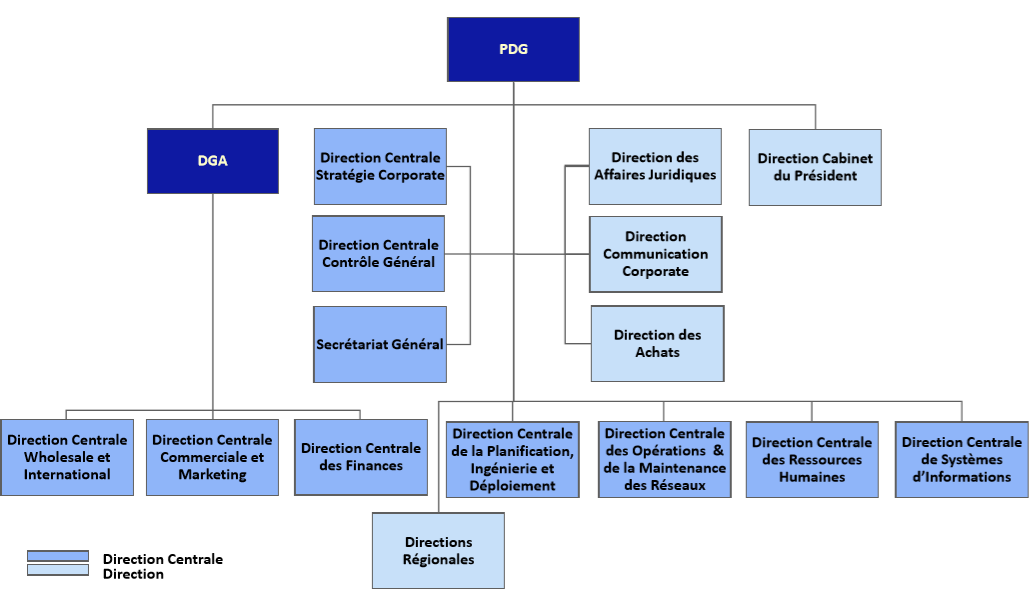
\includegraphics[width=\linewidth]{TT_Hierarchy}
  \caption[TT Hierarchy]{Tunisie Telecom }%\index{Goku il-king}}%
  \label{fig:test1}
\end{figure}

During my internship, I worked for the Data Unit - Business Networks Management Unit that gas the role of ADSL Management, Fiber Optic Management, and management of DATA equipment.

% The belvedere telecommunication complex consists of several centers and services. Following this general presentation, we will move to the precise study of the CC (Switching Center) and the CTN (Digital Transmission Center) where we spent the month of internship.

% Figure 3: Center Structure
% ⦁ Line switching center:

% The CCL is a service that manages the maintenance of the switched network and the installation of transmission cables that connect the subscribers to the central office and the exchanges between them.
% ⦁ Switching Center:

% The Belvedere complex contains two switching exchanges intended to maintain the switching system; The ERICSSON Swedish AX system and the German EWSD system from Siemens. The center is responsible for all subscriber registration operations in the system as well as operations related to fixed telephony services such as prepaid, international calls or caller ID display.
% ⦁ Digital Transmission Center:

% The digital transmission center is one of the basic cells in the telecommunication network. It is the speaker of digital transmission media. In a future chapter of our report, we will take care of his presentation.



% 	This is an Image outlining the Organizational Hierarchy of Tunisie Telecom



\section{Work Environment}
The work environment is exceptionally excellent, Transparent and Open Communication are at the epicenter of what I think is really good about this work environment: We were feeling heard - as interns, we had value and we certainly felt that we belong in the organization. 
They also gave us the opportunity to Give and Take, that is,  we never felt stuck through bureaucracy or even felt that we're doing worthless work, No, our work was at the very center of what Tunisie Telecom employees needed, and we're also allowed to voice our own opinions back, that's a sign of mutual trust in which we're not afraid to suggest ideas to improve the work process! 
And the thing that I truly appreciated about the whole process was the  Recognition of Hard Work: I feel valued by them for the work I had put in.

%\blindtext